\Chapter{Background}

\rule{\textwidth}{2pt}

% Summary of the background material and introduction to the section
The Mastermind puzzle has been subject to investigations regarding solutions to the code-breaking aspect of the game
since its release.
This section will provide background material which aims to give context to the aims and objectives of this project.
The project was inspired by a paper exploring sudoku solutions from a series of problems known as functional pearls,
The processes used to derive those solutions will be used to guide this project in this current stage.
Following this brief introduction is an explanation of the game Mastermind which the solution will be derived from along
with references to previous work by others. The previous work examined will focus on the specific area of search spaces
in regards to finding the optimal best move at each position in the puzzle. At the conclusion of this section the goal is
that the reader has an understanding of the important concepts relating to this project such that the aims and objectives
are clear in their feasibility and relevancy.

\subsection {The Mastermind Puzzle}

The Mastermind puzzle began as a two-player game in which one player seeks to break the code created by the other player \cite{Wolfram}.Originally a physical board game designed by an Isreali Postmaster named Mordecai Meirowitz, distributed through Invicta Toys and Games \cite{Invicta}, the game has evolved into a rich area of investigation due to the strategies
associated with solving its simple rule set.

\subsubsection {The Rules of Mastermind}

% Explanation of Mastermind puzzle
The standard variant of the game as it was introduced in 1970 used a simple plastic board with coloured pegs to represent individual elements for the code.
Each game would begin with a secret code being constructed from c colours and l length, in the standard variant this would result in a code of length four constructed from a set
of six coloured pegs \cite{Wolfram}.

\begin{figure}[H]
\centering
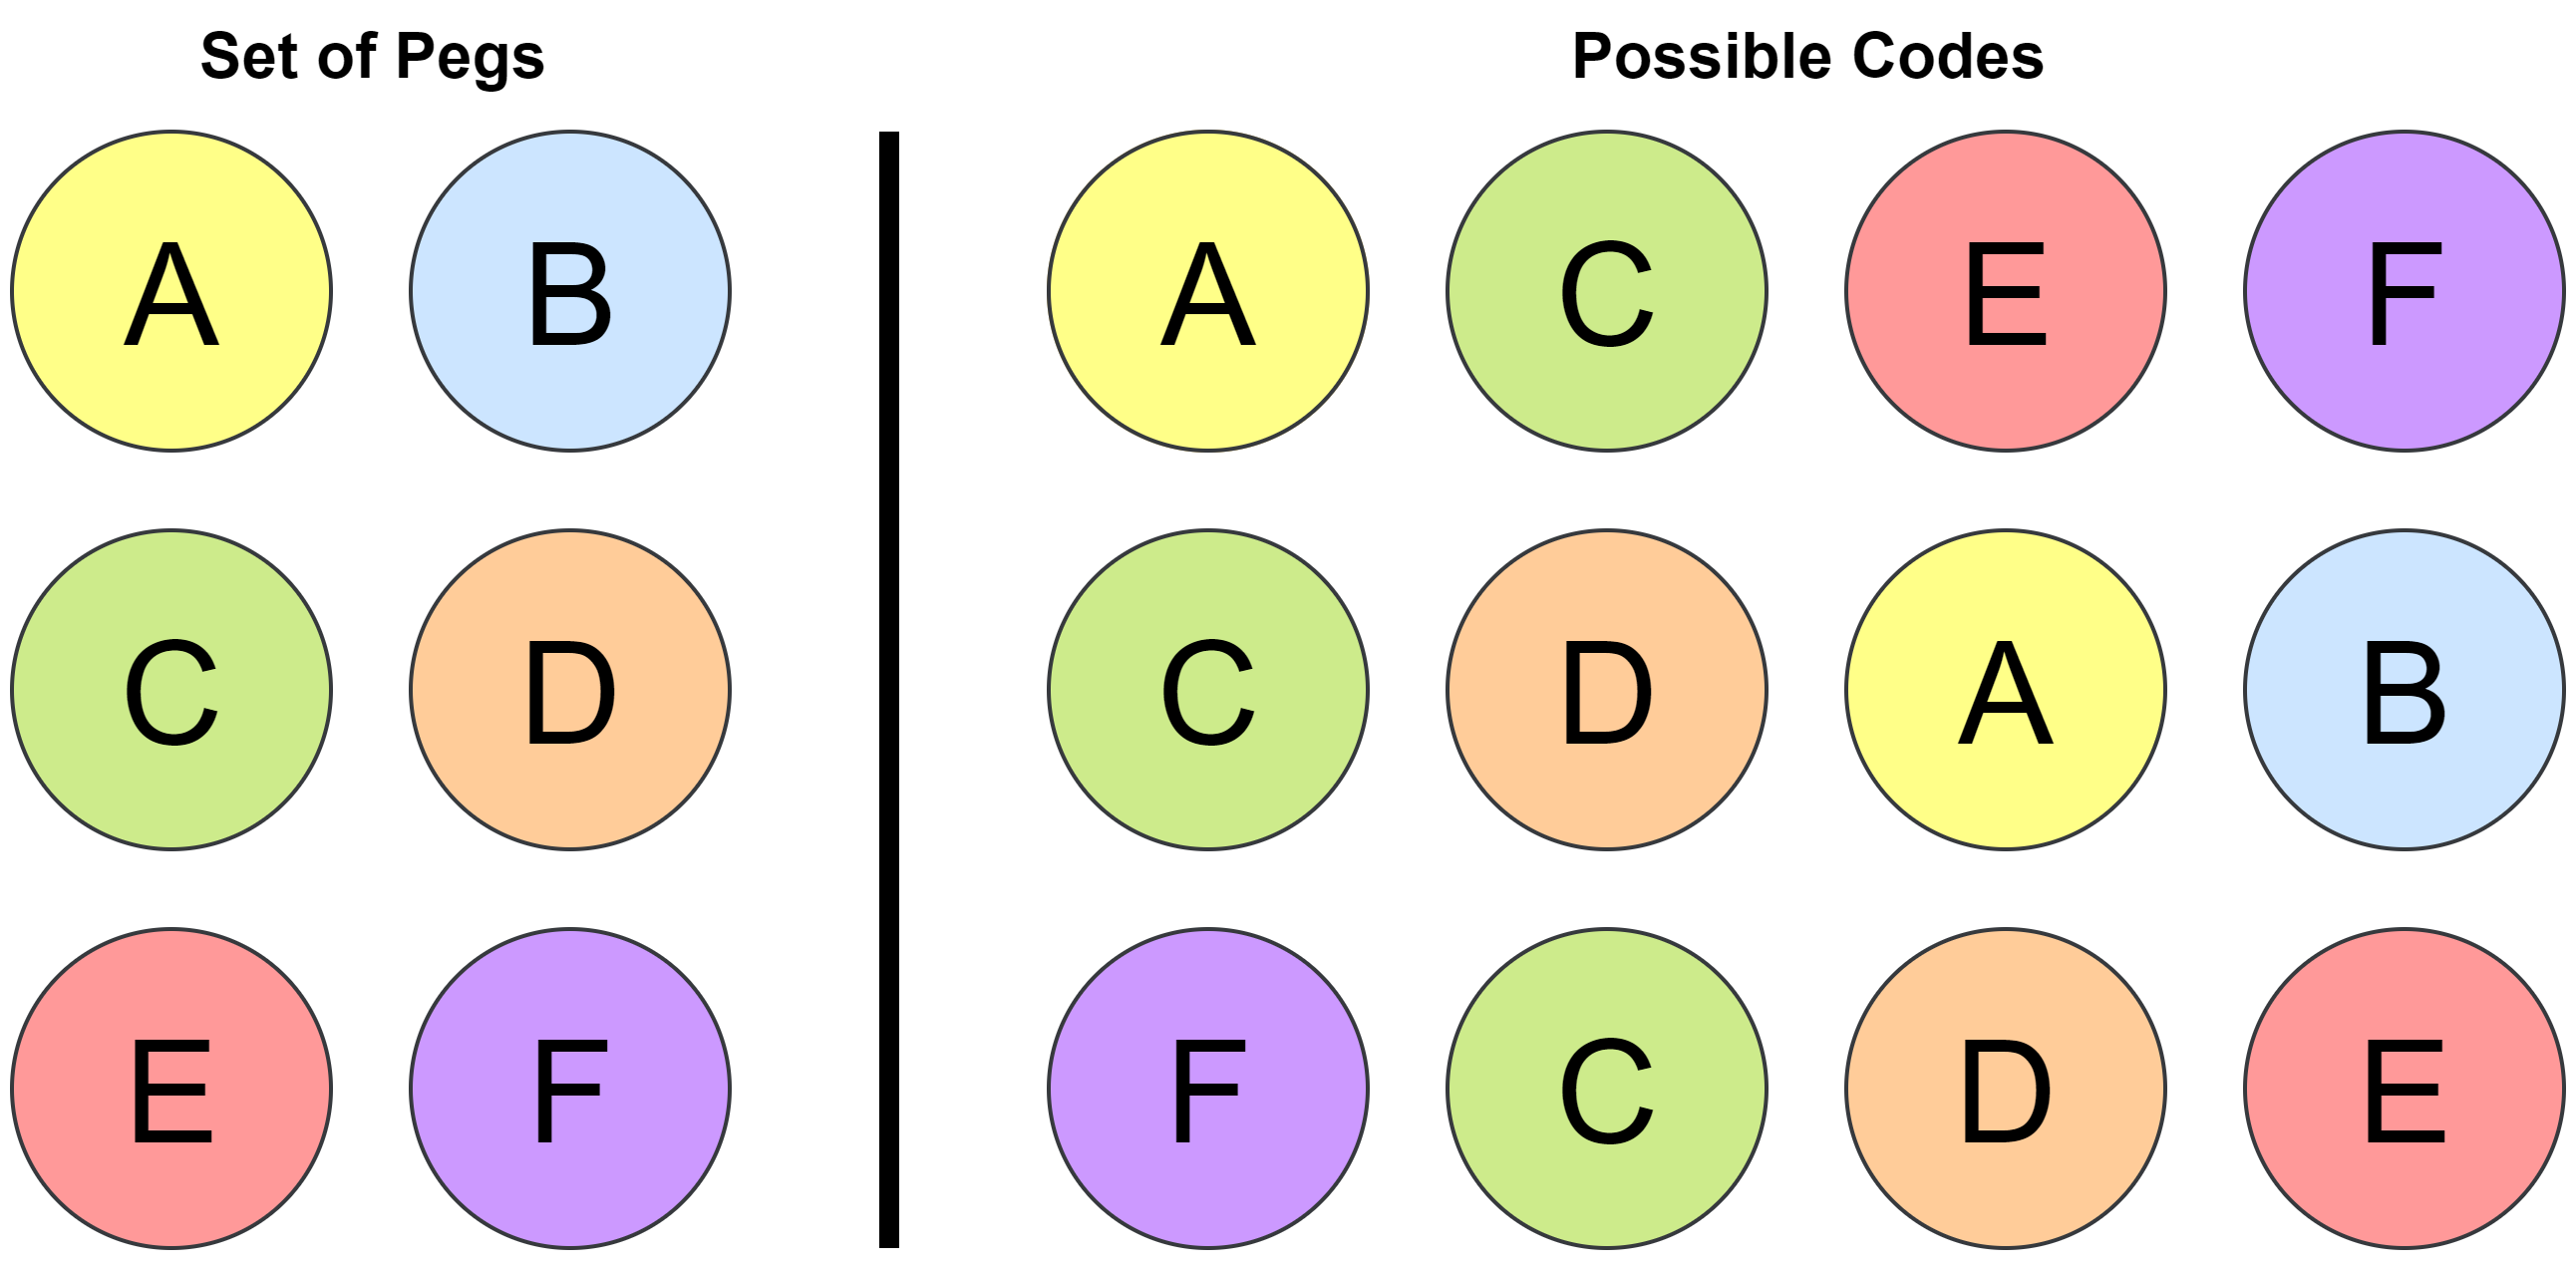
\includegraphics[scale=0.5]{pegs}
\caption{ Example codes which would satisfy the constraints of the standard variant of Mastermind.}
\end{figure}

The codebreaker would attempt several guesses by constructing codes of a similar shape and rewarded with clues as to how closely their guess resembled the hidden code.
The physical game represented these hints as smaller plastic pegs of two colours, one which would denote that a correct colour had been selected but was used in an incorrect
position and one which would confirm that a correct colour and position had been selected for an element.
\begin{figure}[H]
\centering
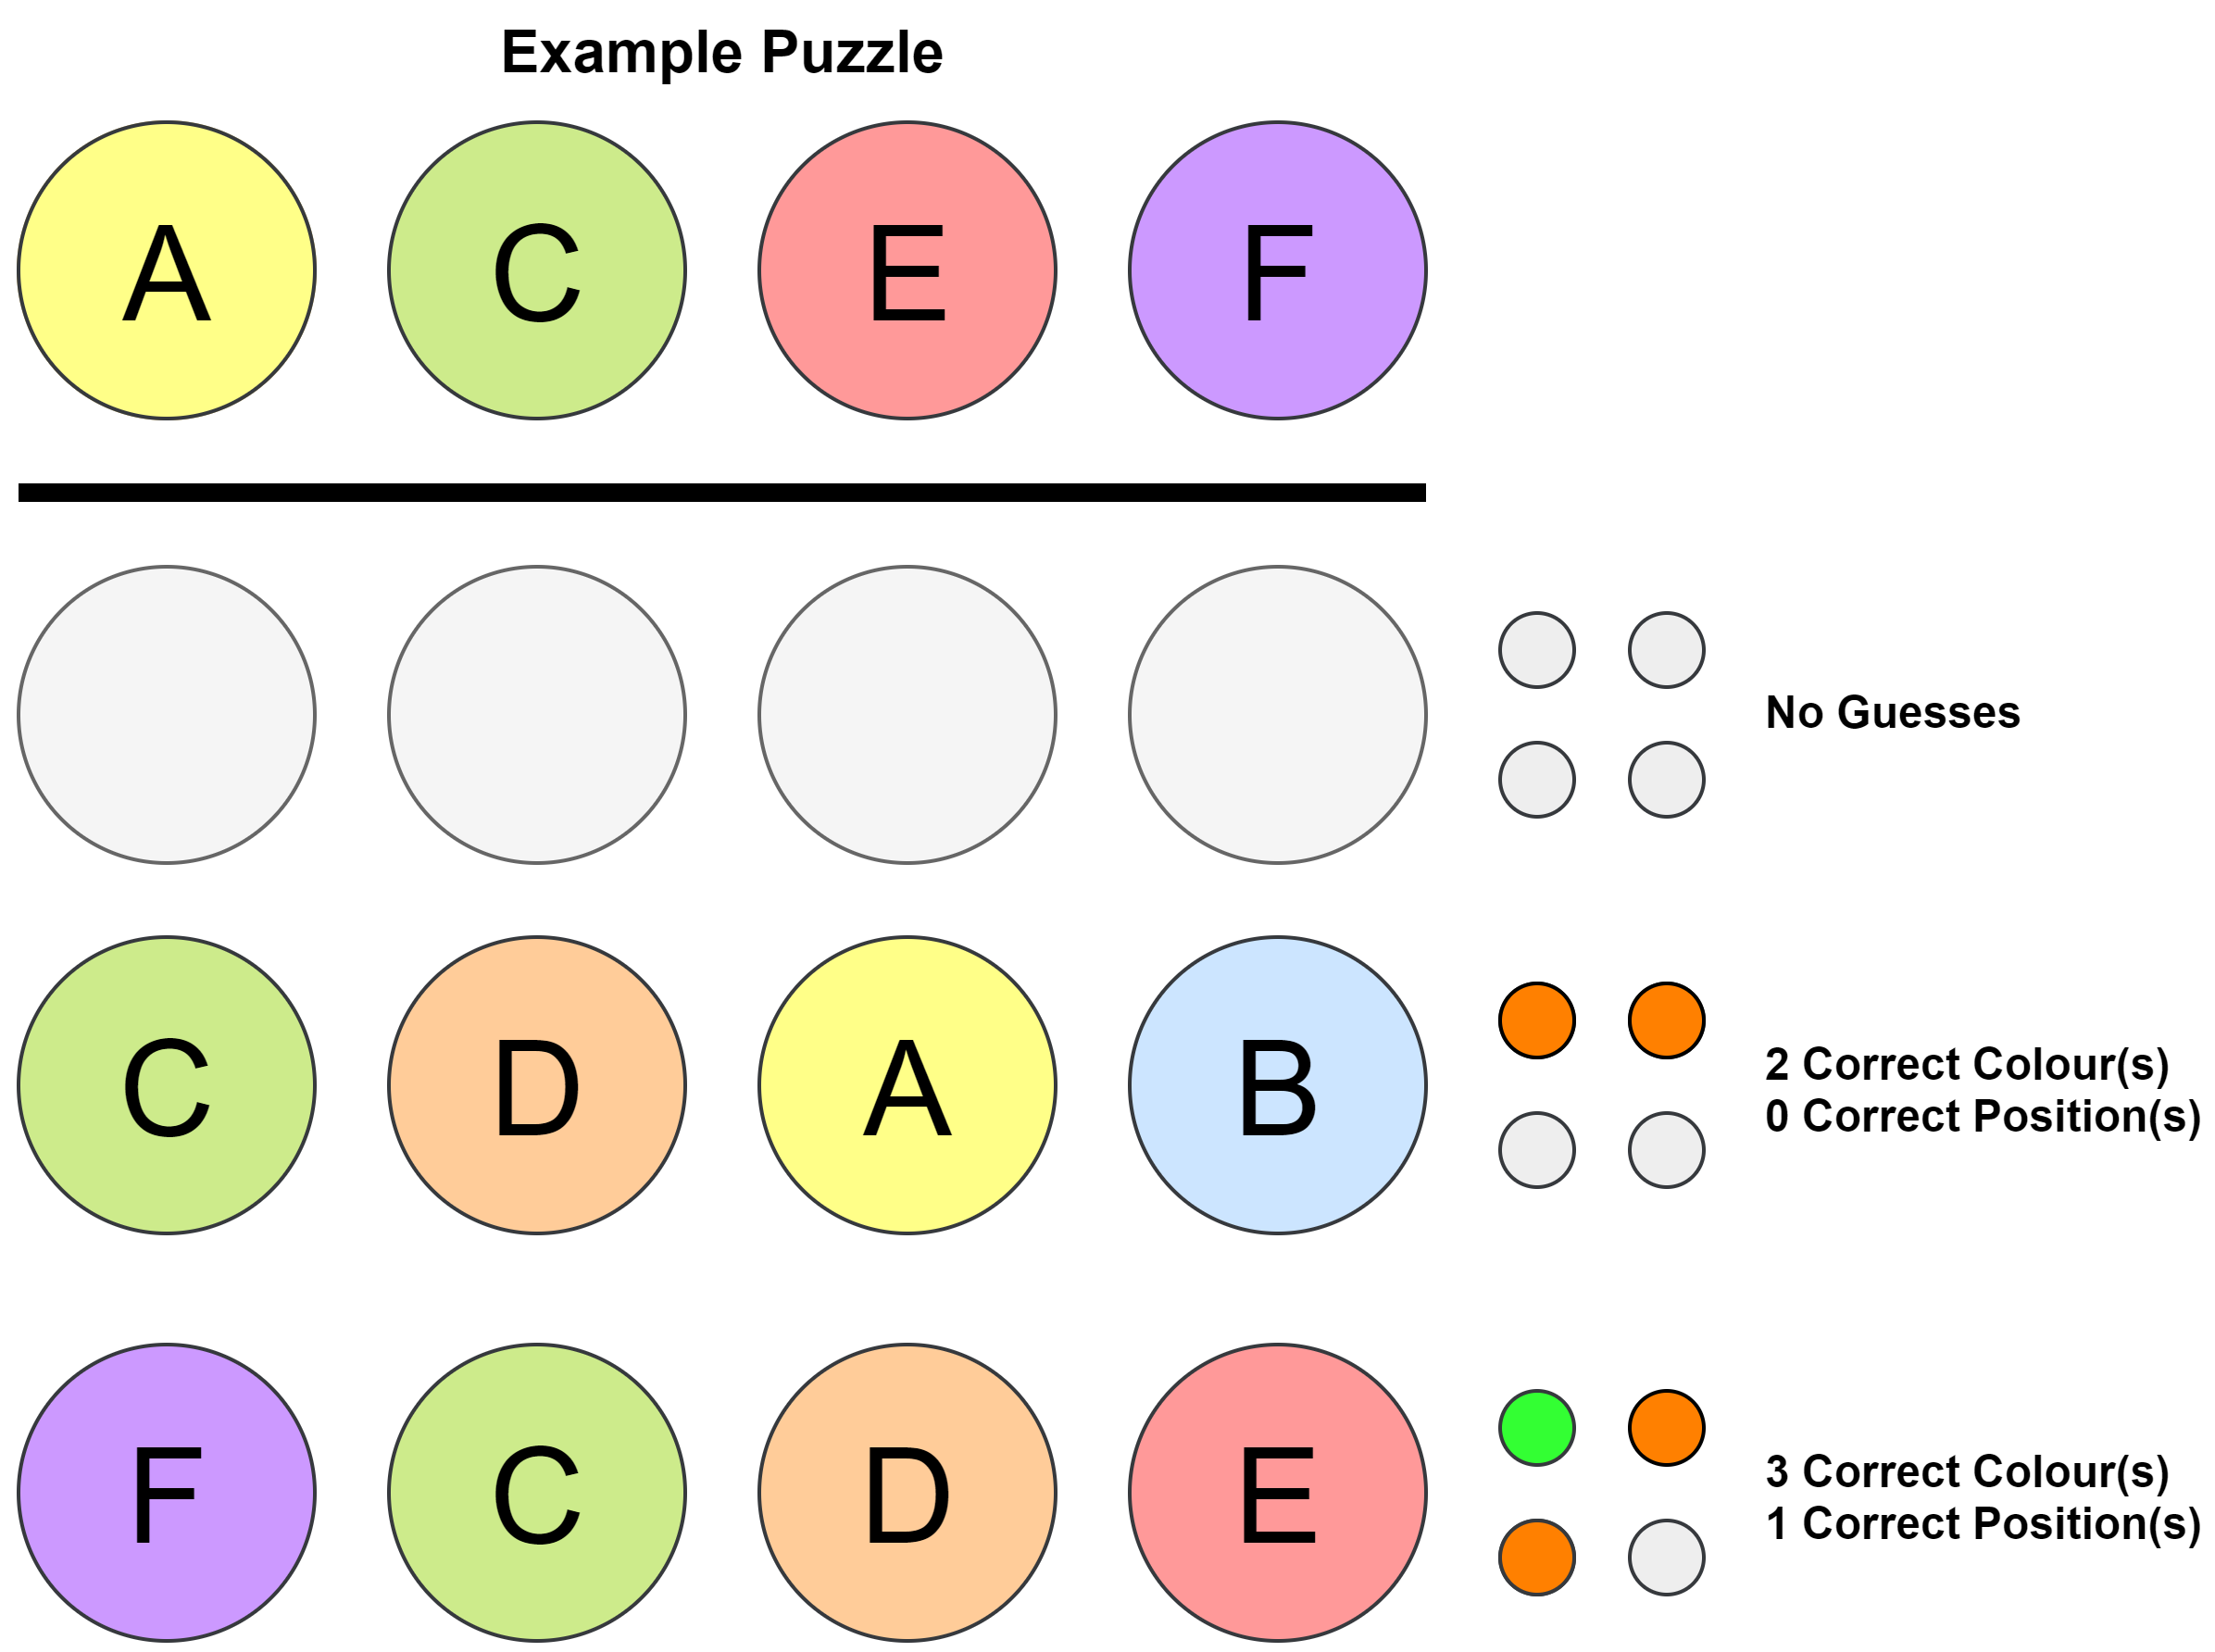
\includegraphics[scale=0.5]{guesses}
\caption{A simplified representation of $CB$ attempting to break the code set by $CM$}
\end{figure}

There are two end states of the game, one in which the code is broken and discovered by the guessing player and one in which the guessing player is unable to discover the code
within a limit of guesses.
